\chapter{Supporting Figures}
\label{app:figures}

The figures below support the text of Chapters~1 and~3, where each is referenced.

\begin{figure}[htbp]
\centering
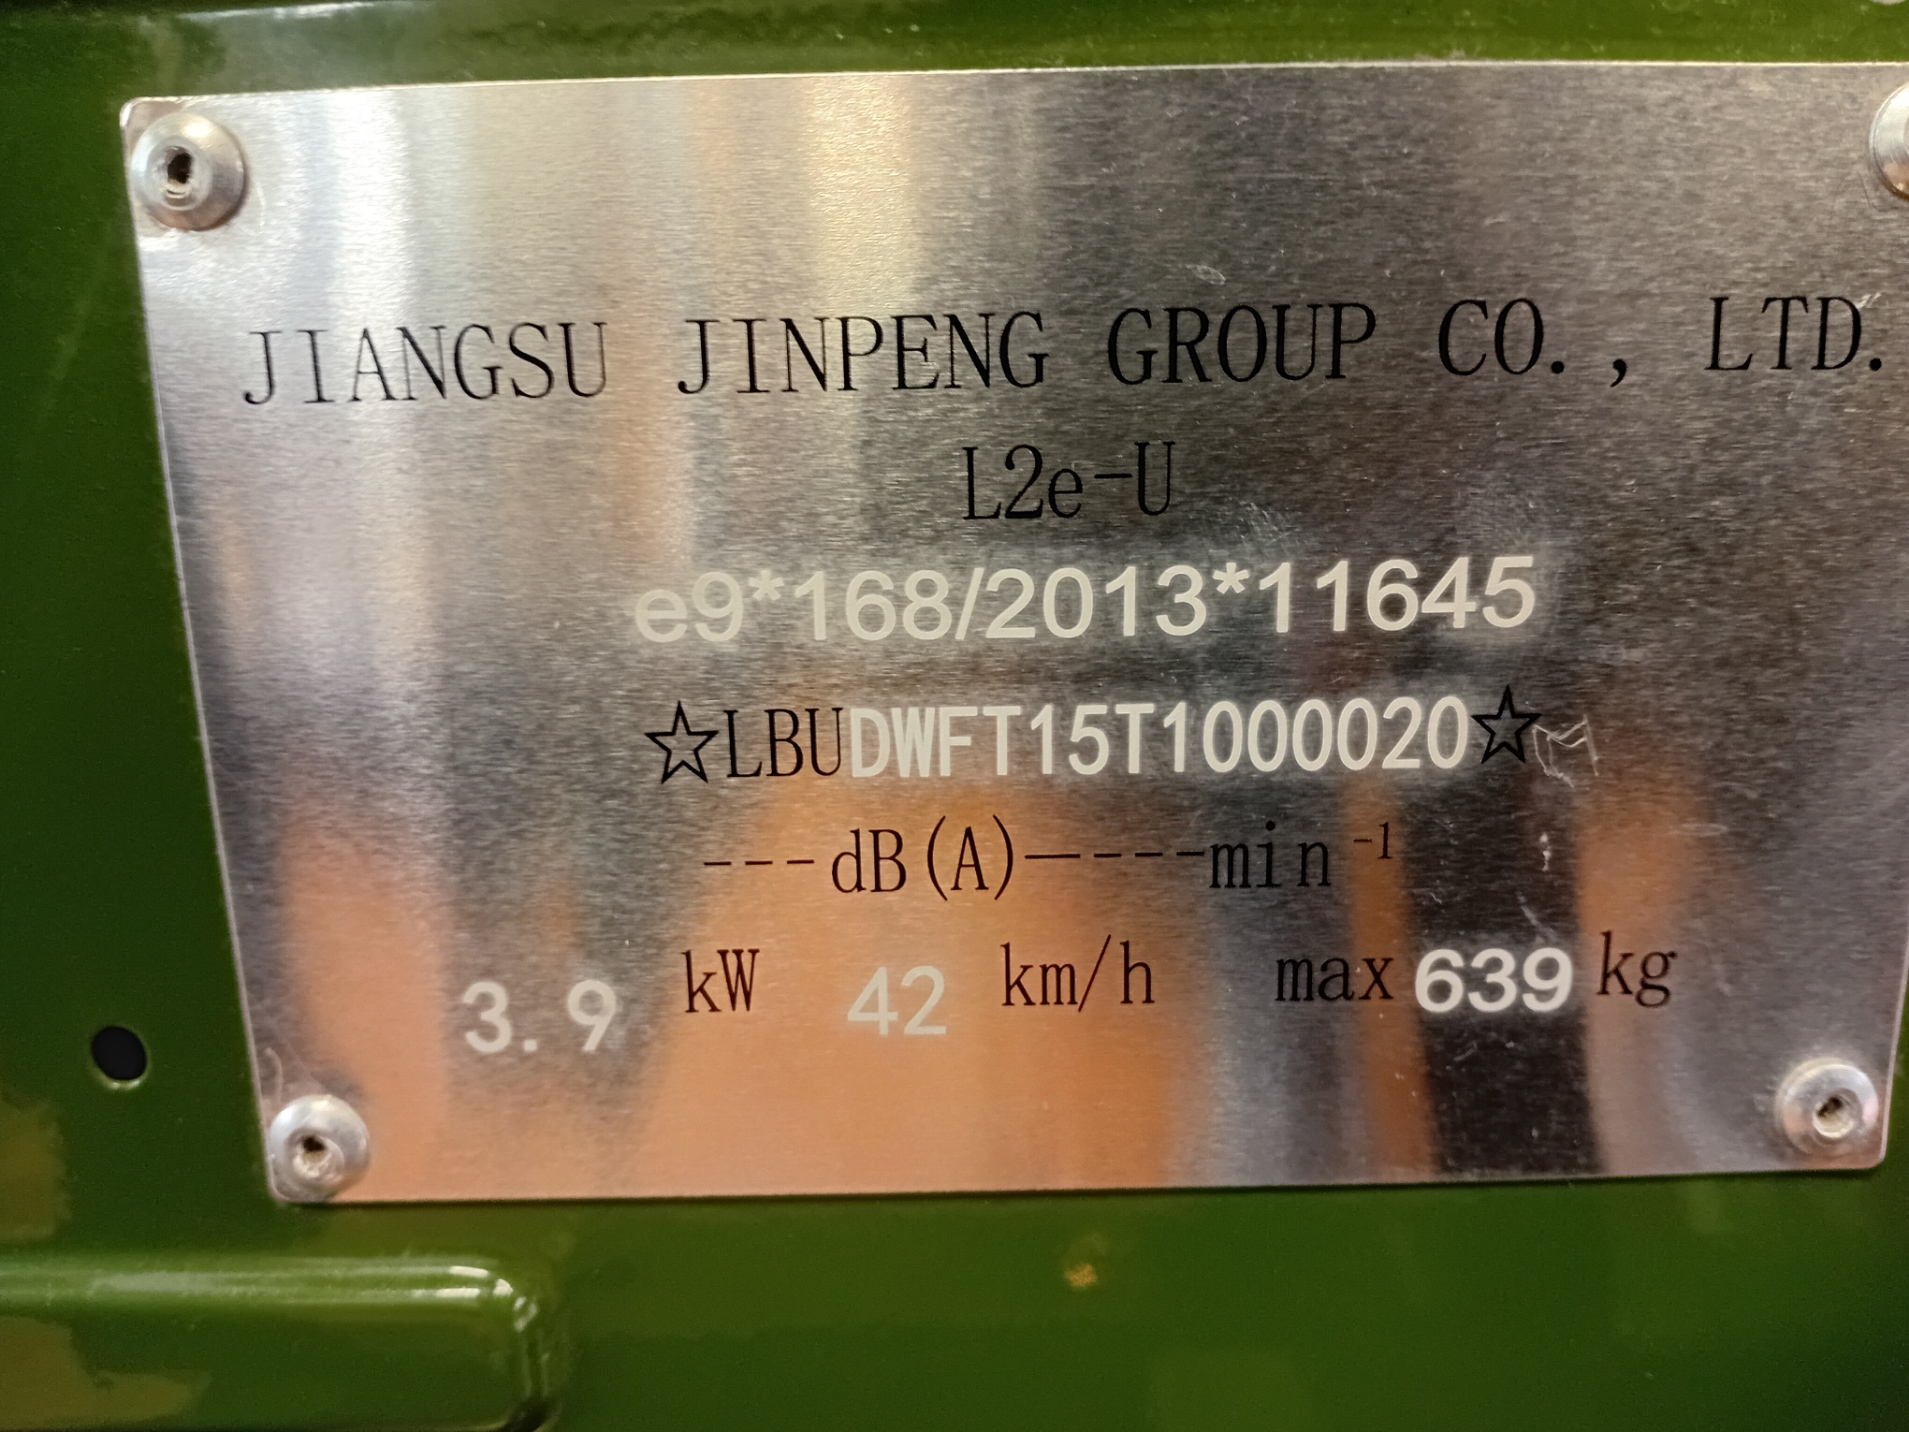
\includegraphics[width=0.55\textwidth]{figures/vehicle_nameplate.jpg}
\caption{Manufacturer identification plate on the TUKZIE Rev 0 platform, photographed directly during vehicle inspection.}
\label{fig:vehicle-nameplate}
\end{figure}

\begin{figure}[htbp]
\centering
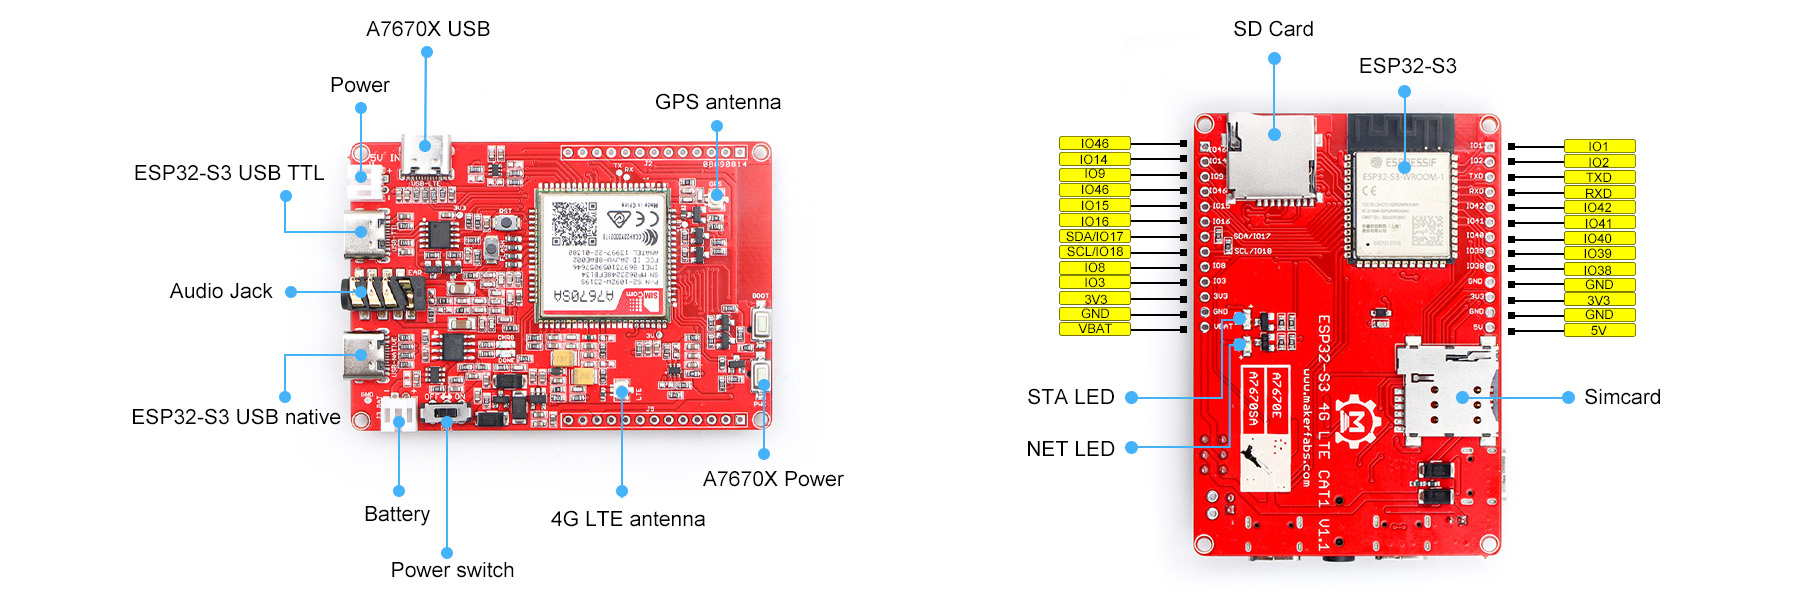
\includegraphics[width=\textwidth]{figures/makerfabs_a7670x_pinout.jpg}
\caption{Makerfabs ESP32-S3 4G LTE CAT1 A7670X board: manufacturer-labelled ports (left) and pinout (right) \cite{makerfabsa7670x}.}
\label{fig:makerfabs-pinout}
\end{figure}

\begin{figure}[htbp]
\centering
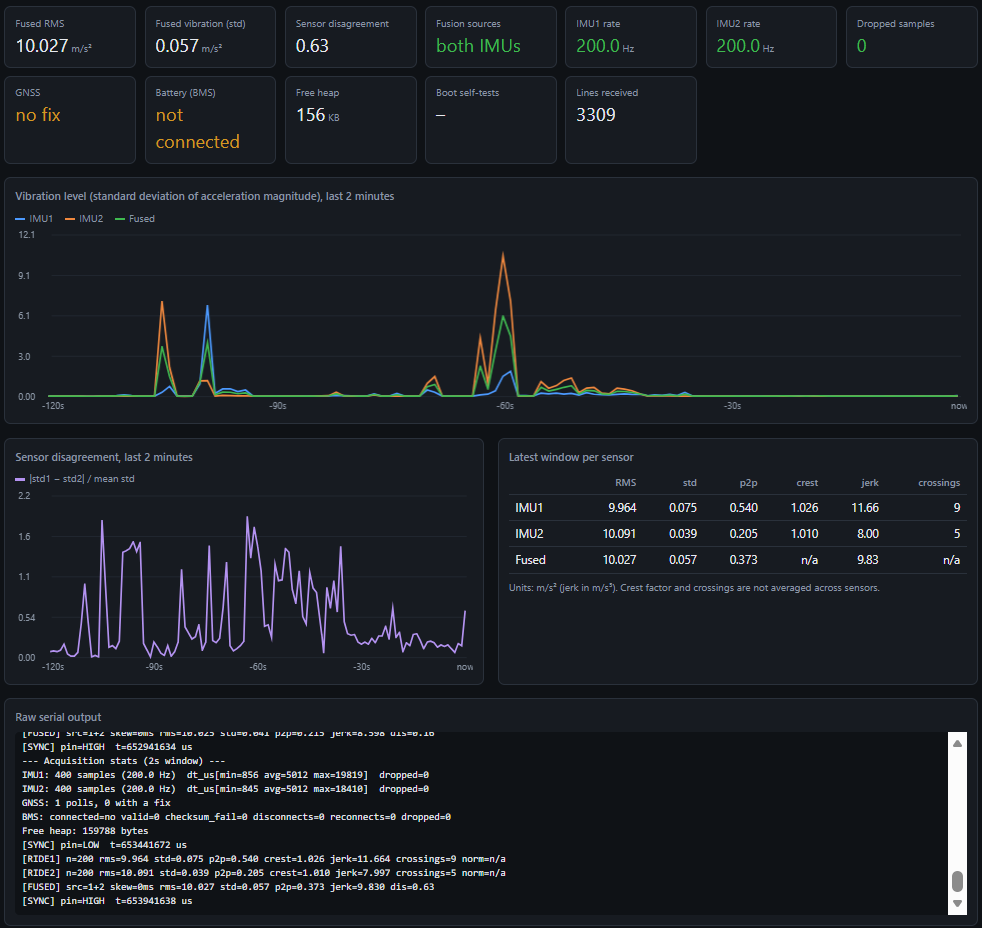
\includegraphics[width=0.85\textwidth]{figures/live_dashboard.png}
\caption{The live telemetry dashboard connected to the telemetry unit over USB during bench testing, showing both IMUs fused at 200\,Hz with no dropped samples and two hand disturbances in the vibration plot.}
\label{fig:live-dashboard}
\end{figure}

\begin{figure}[htbp]
\centering
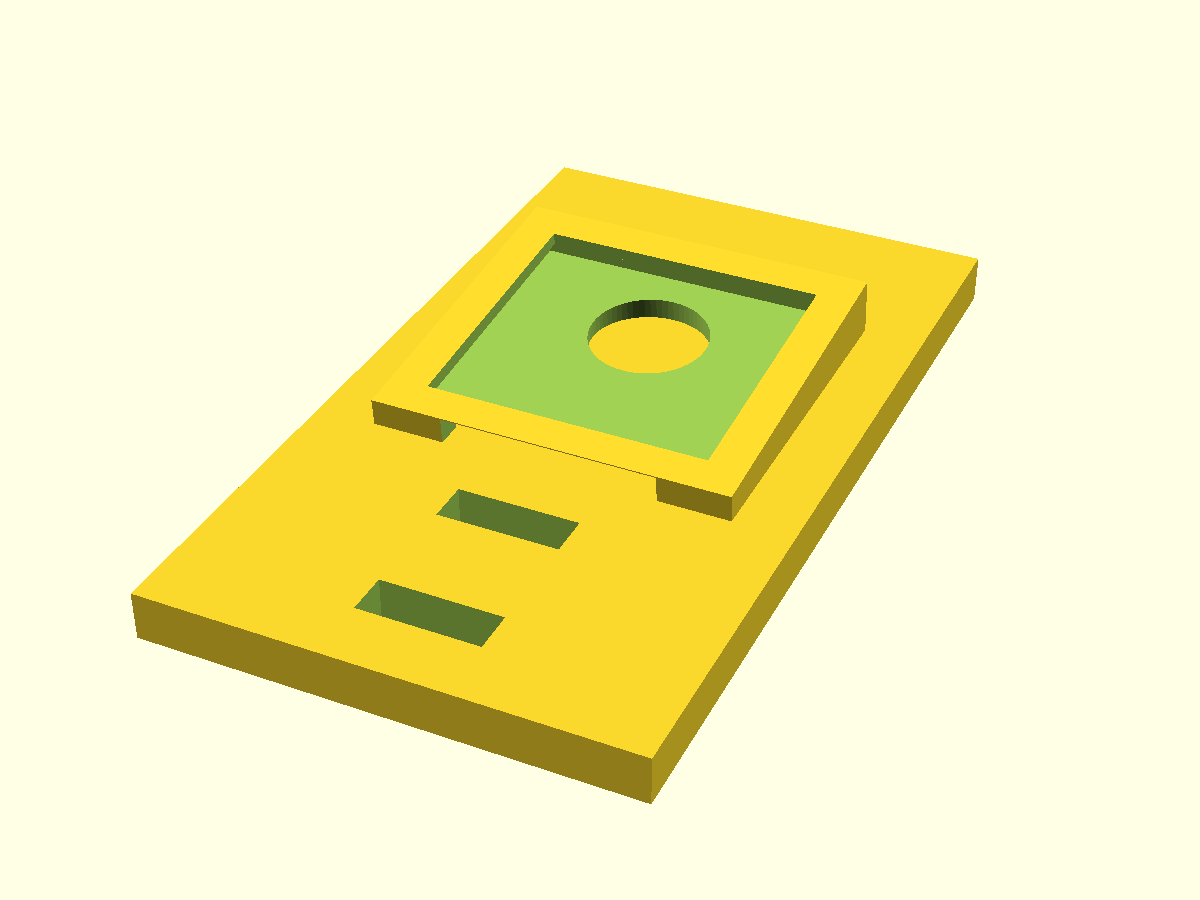
\includegraphics[width=0.6\textwidth]{figures/camera_mount_render.png}
\caption{Initial parametric camera bracket (OpenSCAD, full render), showing the corrected lens-retention lip and cable-routing slots. This design was not printed.}
\label{fig:camera-mount}
\end{figure}
